\chapter{Electric / Hybrid RV Propulsion}
\section{Introduction}
\subsection{Reasons forcing change}
\begin{itemize}
    \item Global warming e.g. CO2 emissions
    \item Health e.g. NOx emissions
    \item Efficiency e.g. low efficiency of vehicles presently
    \item Technology advances e.g. batteries
    \item Increasing demand e.g. in developing countries
    \item Custom demand e.g. environmental concerns
\end{itemize}
\subsection{Global CO2 emissions}
\begin{figure}[H]
    \centering
    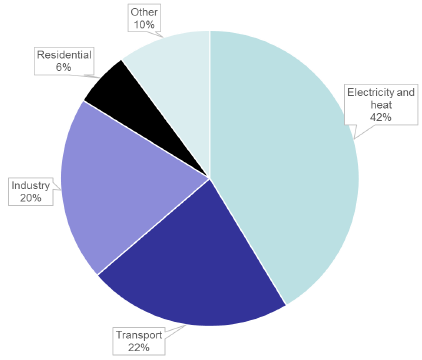
\includegraphics[width = 0.8\textwidth]{img/figure92.png}
    \caption{Global CO2 emissions.}
\end{figure}
Transport is a significant contribution to CO2 global emissions. It is a bigger emitter than electricity generation in many countries.
\subsection{Typical driving energy losses (city use)}
\begin{figure}[H]
    \centering
    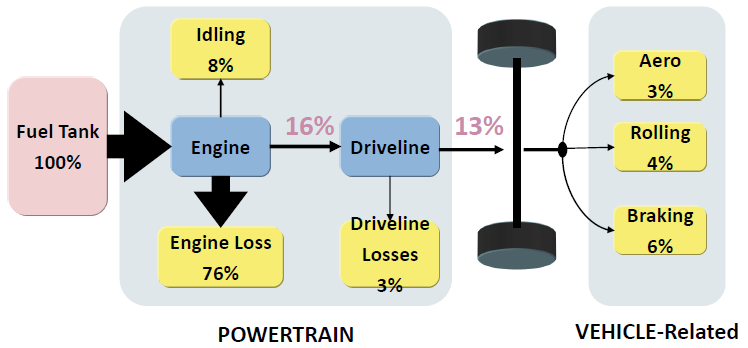
\includegraphics[width = 0.8\textwidth]{img/figure93.png}
    \caption{Typical driving energy losses (city use).}
\end{figure}
The efficiency of ICE engines in road vehicles is low.
\subsection{Transport sector growth prediction}
\begin{figure}[H]
    \centering
    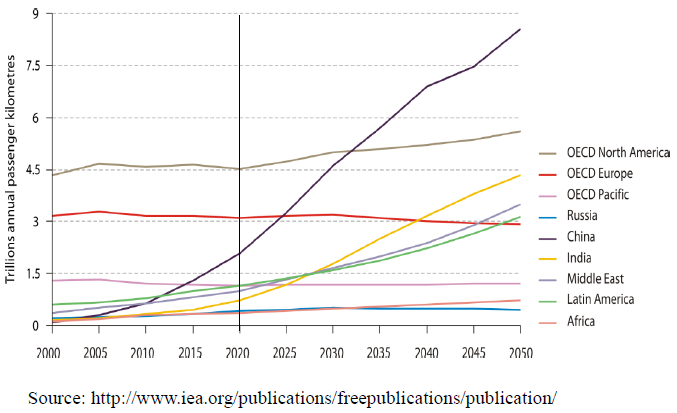
\includegraphics[width = 0.8\textwidth]{img/figure94.png}
    \caption{Transport sector growth prediction.}
\end{figure}
Transport growth is mainly in developing countries whereas developed countries are expected to remain unchanged.
\subsection{Gasoline: the (almost) perfect fuel}
\begin{figure}[H]
    \centering
    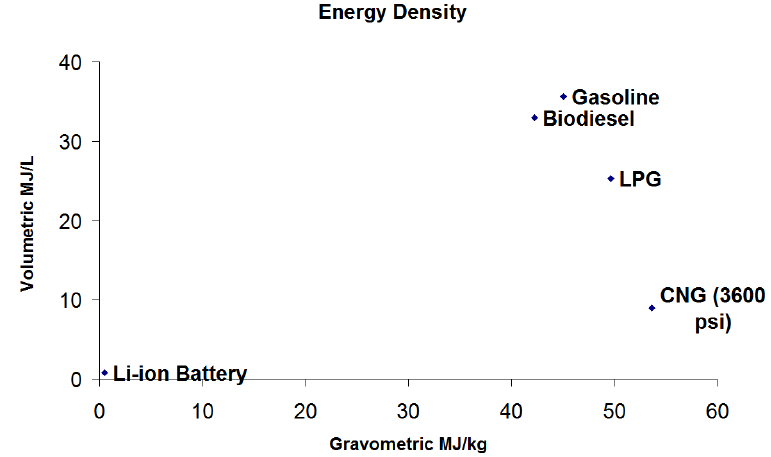
\includegraphics[width = 0.8\textwidth]{img/figure95.png}
    \caption{Transport sector growth prediction.}
\end{figure}
\subsection{Towards zero emissions}
\begin{figure}[H]
    \centering
    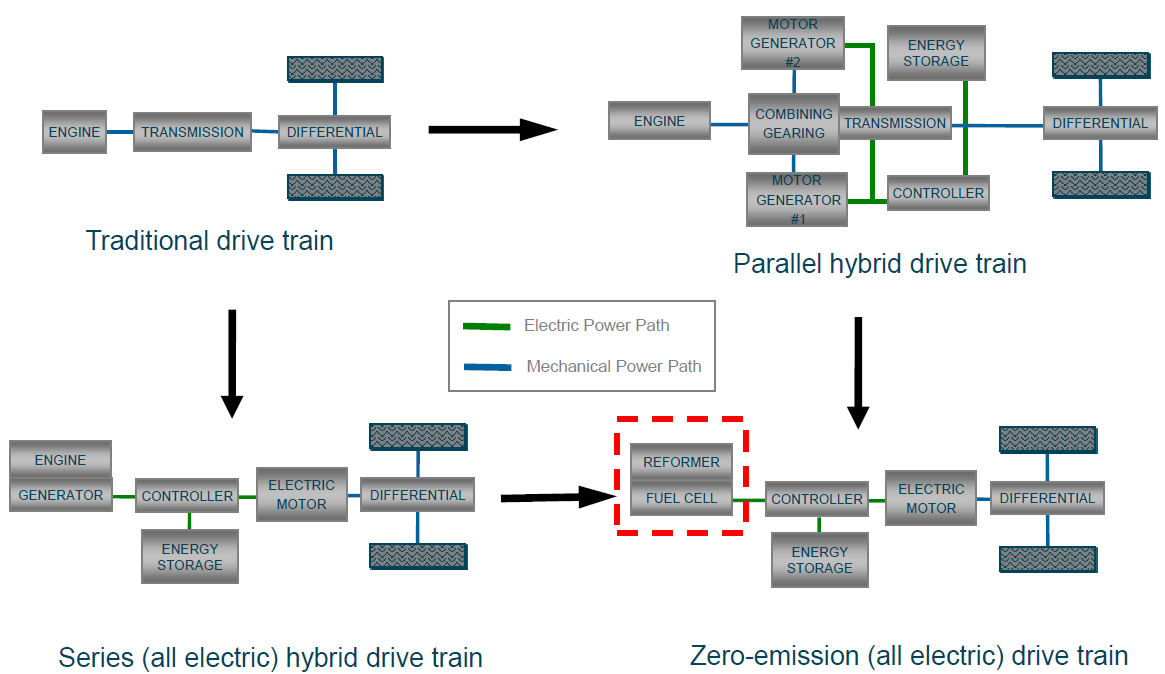
\includegraphics[width = 0.8\textwidth]{img/figure96.png}
    \caption{Drive trains for various vehicle types.}
\end{figure}
\section{Hybrid vehicles}
\subsection{Growth of hybrid and battery vehicles}
\begin{figure}[H]
    \centering
    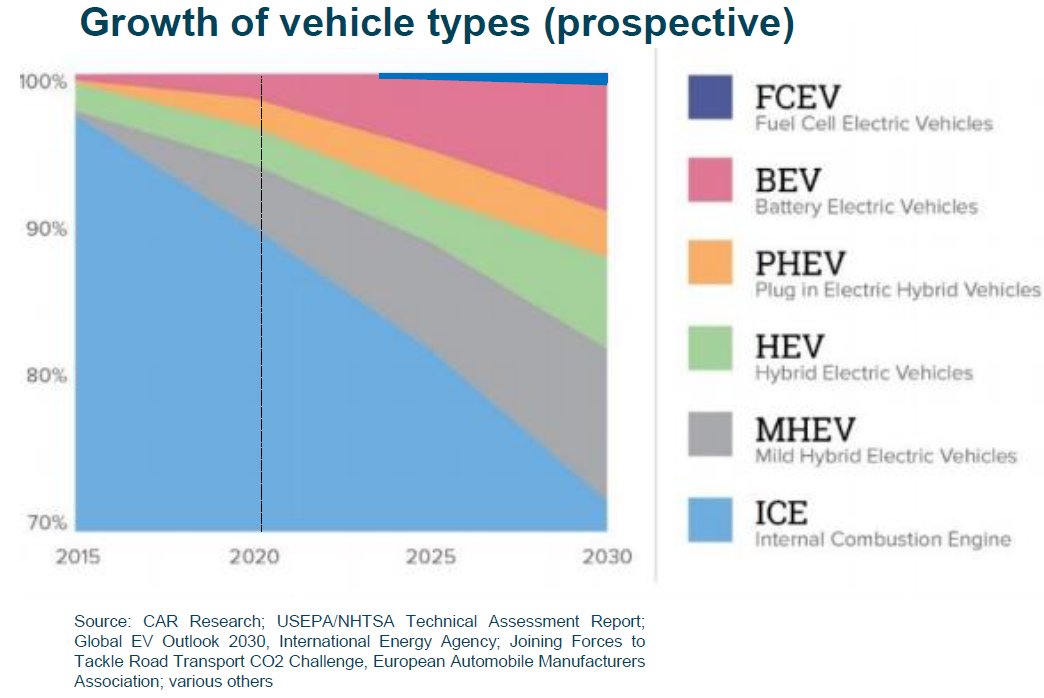
\includegraphics[width = 0.8\textwidth]{img/figure97.png}
    \caption{Growth of vehicle types (prospective).}
\end{figure}
\subsection{Hybrid types}
\begin{figure}[H]
    \centering
    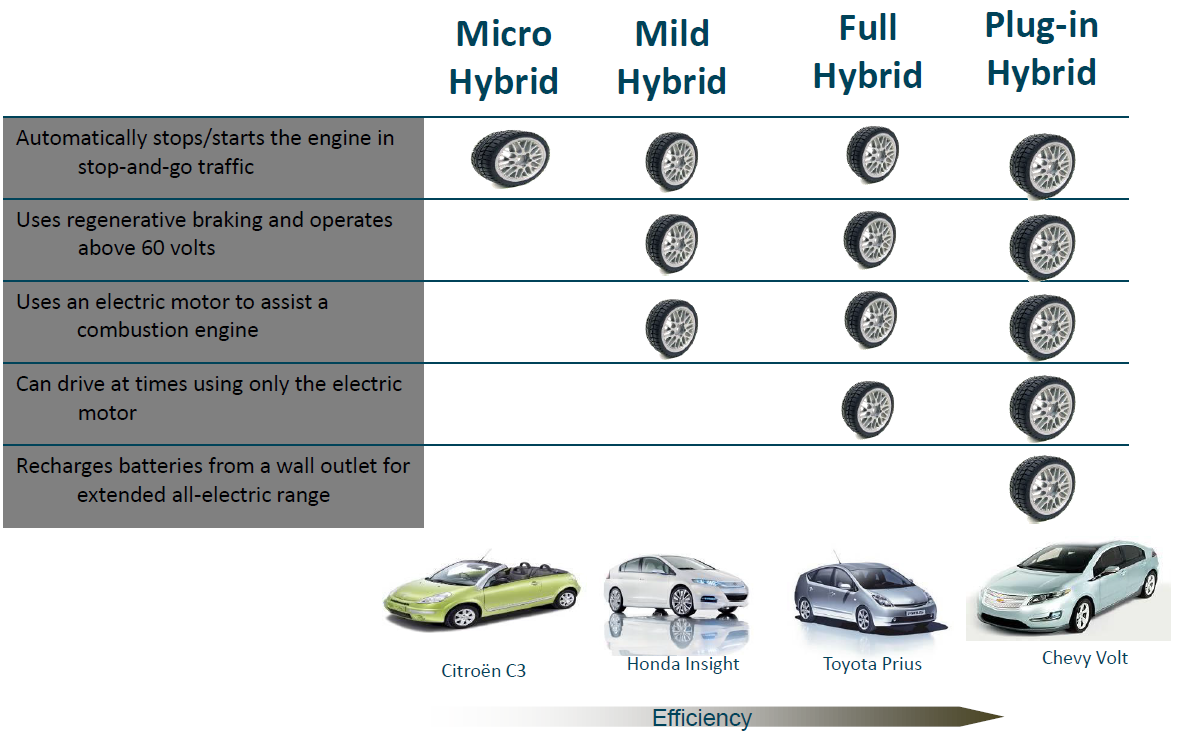
\includegraphics[width = 0.8\textwidth]{img/figure98.png}
    \caption{Hybrid types.}
\end{figure}
\subsection{Typical hybrid: city driving energy loss}
\begin{figure}[H]
    \centering
    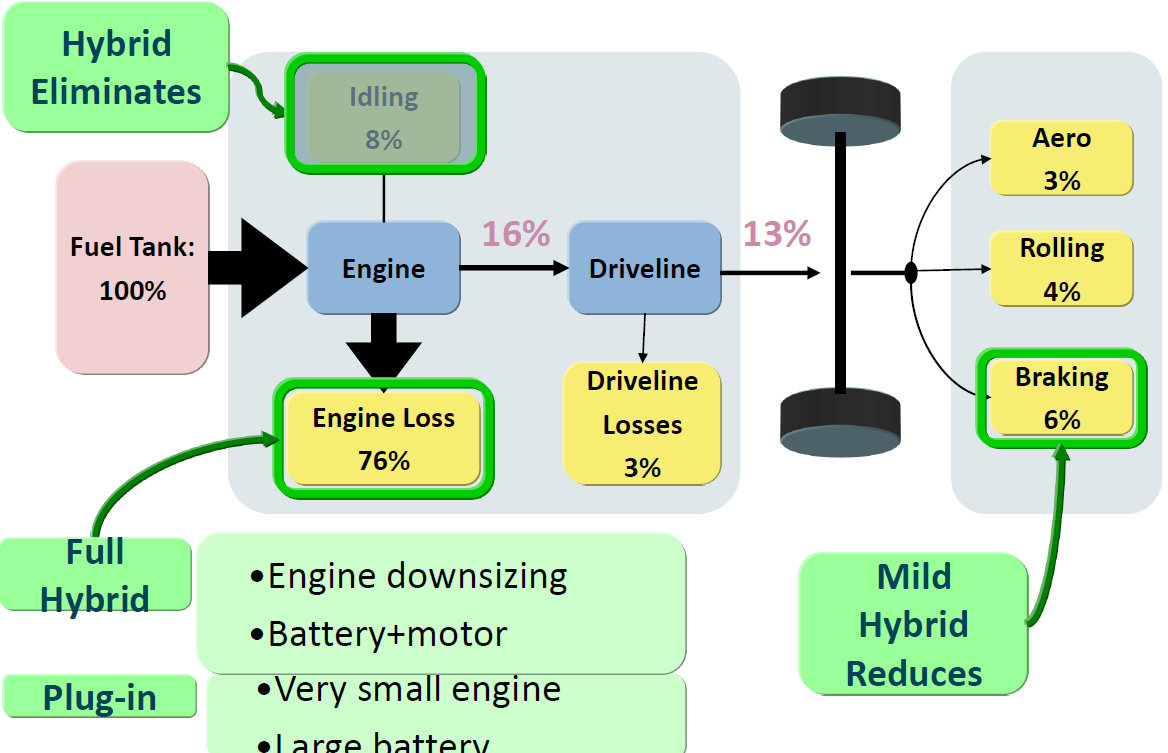
\includegraphics[width = 0.8\textwidth]{img/figure99.png}
    \caption{Typical hybrid: city driving energy loss.}
\end{figure}
\subsection{Types of hybrid arrangements}
\begin{figure}[H]
    \centering
    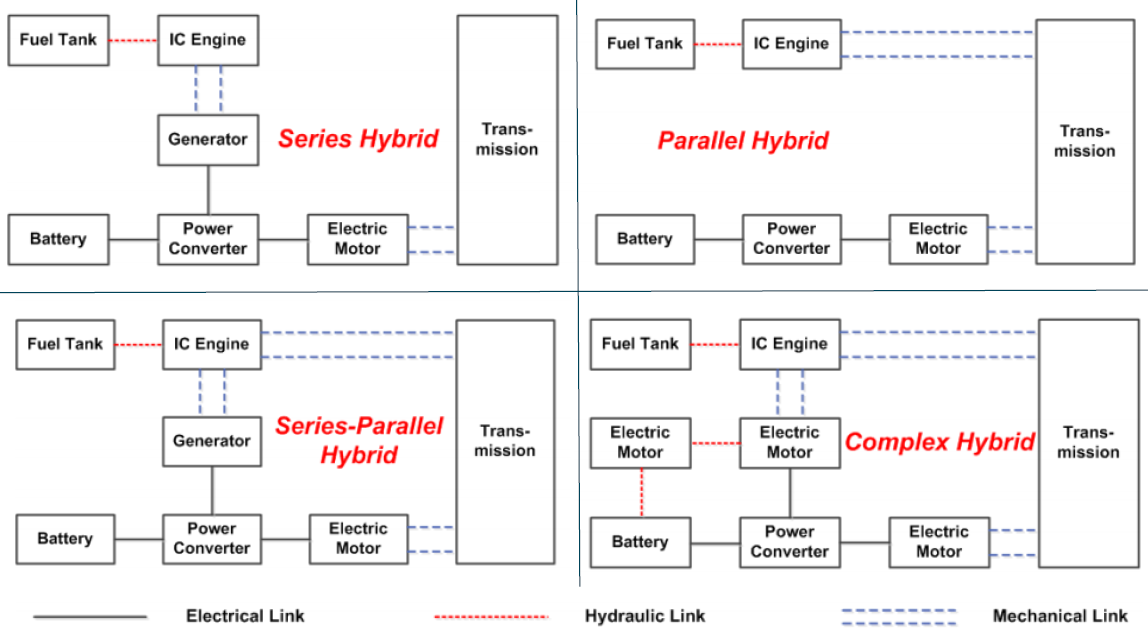
\includegraphics[width = 0.8\textwidth]{img/figure100.png}
    \caption{Types of hybrid arrangement.}
\end{figure}
\subsection{Regenerative braking}
\begin{figure}[H]
    \centering
    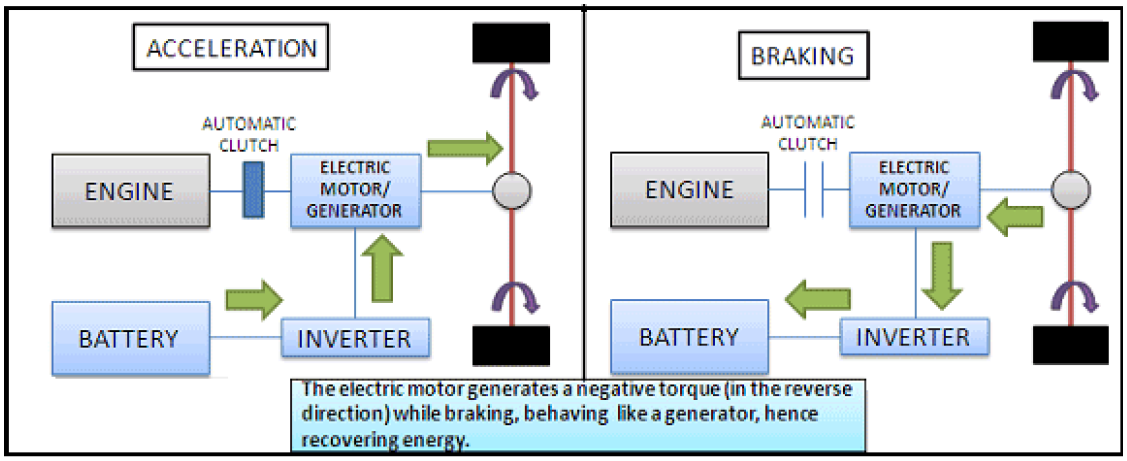
\includegraphics[width = 0.8\textwidth]{img/figure101.png}
    \caption{Regenerative braking.}
\end{figure}
Regenerative braking allows energy to be collected by the battery. In practice a mechanical brake is also needed.
\subsection{Example: arrangement for hybrid bus}
\begin{figure}[H]
    \centering
    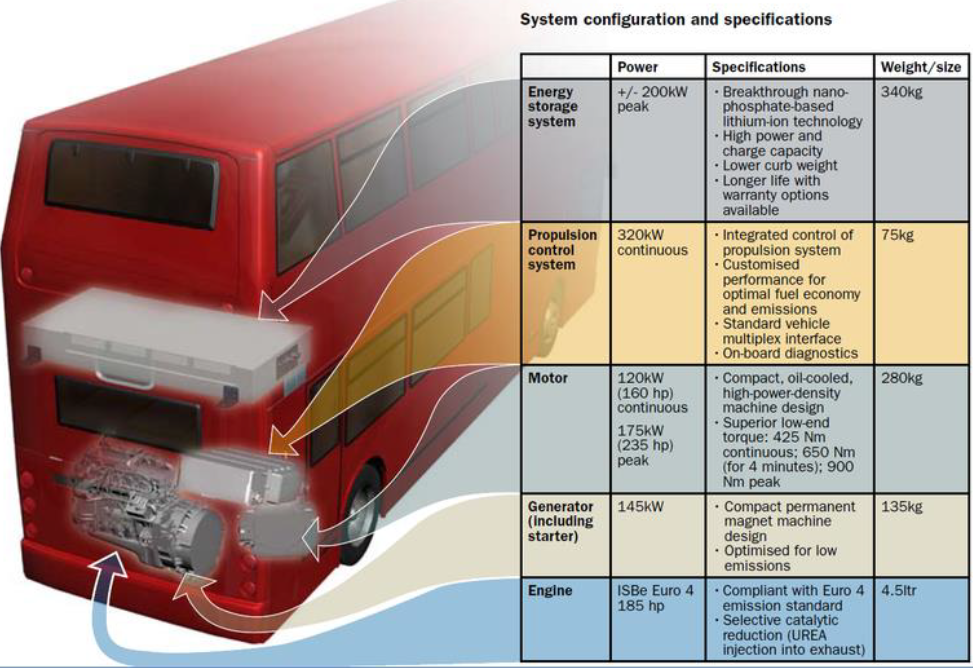
\includegraphics[width = 0.8\textwidth]{img/figure102.png}
    \caption{Example: arrangement for hybrid bus.}
\end{figure}
\subsection{Complete diesel-generator-motor power plant assembly}
\begin{figure}[H]
    \centering
    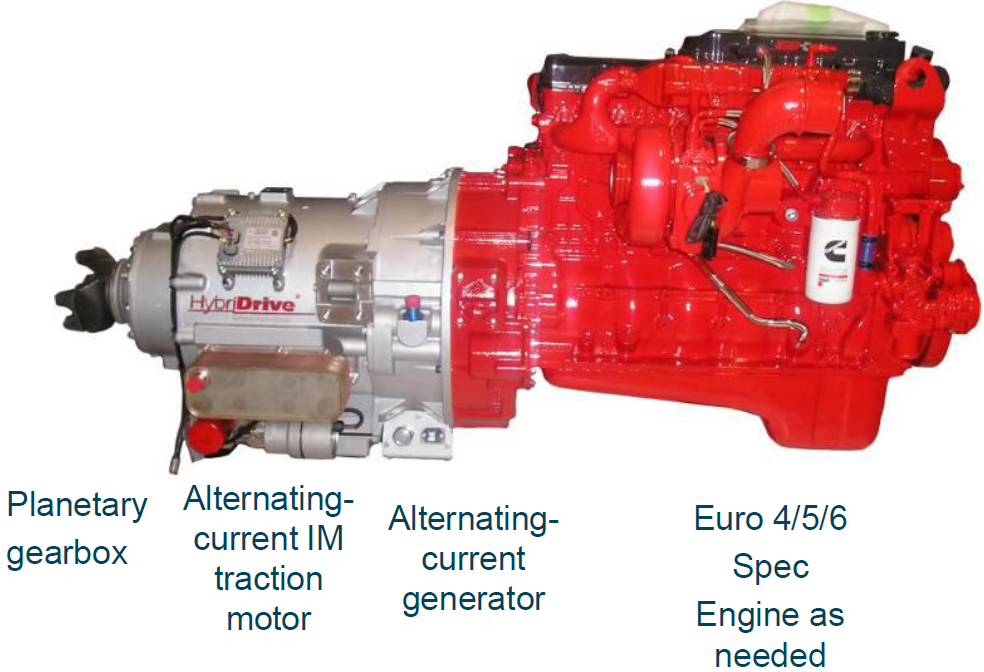
\includegraphics[width = 0.8\textwidth]{img/figure103.png}
    \caption{Complete diesel-generator-motor power plant assembly.}
\end{figure}
\subsubsection{Traction generator}
\begin{itemize}
    \item Power rating: \SI{200}{\kilo\watt} continuous at \SI{2300}{rpm}
    \item Liquid cooled
\end{itemize}
Features:
\begin{itemize}
    \item Integrated starter
    \item Brushless permanent magnet
    \item High power to weight ratio
    \item Fully sealed and liquid cooled - meets international standard (IP67)
    \item Standardised interface to engine
\end{itemize}
Benefits:
\begin{itemize}
    \item Quieter start
    \item Eliminates starter motor and flywheel
    \item Minimal maintenance
    \item Inexpensive across a hybrid fleet
\end{itemize}
\subsubsection{Modular traction system}
\begin{itemize}
    \item Vehicle installation flexibility: inline of transverse
    \item IM for robustness and flexibility
    \item Meets all industry top speed, acceleration and gradient performance requirements
    \item Designed to fit in conventional transmission footprint
    \item Variable speed with reduction gearbox to keep m/c size optimal
\end{itemize}
\subsection{Advanced lithium-ion energy storage system}
\begin{figure}[H]
    \centering
    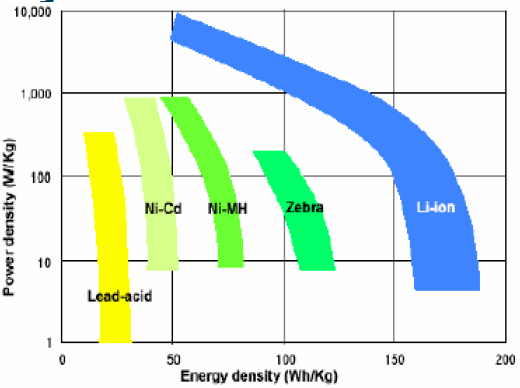
\includegraphics[width = 0.8\textwidth]{img/figure104.png}
    \caption{Energy density of various battery technologies.}
\end{figure}
Lithium advantages:
\begin{itemize}
    \item Weight: 400kg
    \item Life: 6-8 years
    \item Reliability: fault-tolerant
    \item Service: modular design
\end{itemize}
\begin{itemize}
    \item Ambient air cooled
    \item Improvement over lead acid batteries
    \item Best power and energy density
    \item Lower weight
    \item Long battery life - reduces life cycle cost
\end{itemize}
\subsection{Electrical auxiliaries}
A suite of electric accessories including:
\begin{itemize}
    \item Electric power steering
    \item Hydraulic systems
    \item Driver aircon system
    \item Engine cooling fans
    \item Diesel engine stop/start
\end{itemize}
\subsection{Optional system cooling package}
Features:
\begin{itemize}
    \item Integrated water ethylene glycol-based cooling system
          \begin{itemize}
              \item Optimised for HybriDrive heat rejections
          \end{itemize}
    \item Flexible horizontal and vertical mounting options
    \item Two \SI{28}{\volt} DC electric fans
    \item One \SI{28}{\volt} DC electric centrifugal water pump
    \item \SI{8.5}{fins/inch} transit rated radiator core
    \item Built-in fluid level sensor
    \item SAE J1939 CAN-based pump power. pump speed and WEG temperature feedback
    \item Active overflow reservoir allows automatic cooling loop deaeration (active bleed)
    \item \SI{5}{psi} reservoir bottle
    \item Sized for system coolant volume of 5 gallons
\end{itemize}
Benefits:
\begin{itemize}
    \item Provides optimal `drop-in' cooling solution
    \item Built in sensors and flow detection for protection
    \item Fully integrated with HybriDrive control laws
    \item Greater reliability and increased life through optimal temperature control
    \item Ease of maintenance
    \item Fully electric accessories provide on-demand cooling for better overall system efficiency
    \item Fully electric accessories allows for engine shutdown
\end{itemize}
\subsection{Propulsion control system}
\begin{itemize}
    \item Power rating: 2 $\times$ \SI{200}{\kilo\watt} continuous
    \item Coolant: WEG \SI{15}{gpm}
\end{itemize}
Features:
\begin{itemize}
    \item Selectable acceleration and braking settings
    \item Minimal internal interconnects
    \item Onboard diagnostics
    \item SAE 1939 CAN interface
    \item Control electronics mounted externally
    \item Optional DC output to support electric heater or brake resistor
    \item BAE Systems cooling system option available to OEM
\end{itemize}
Benefits:
\begin{itemize}
    \item Rugged, durable and highly reliable
    \item Flexibility of installation and cooling
    \item Standard communications interface
    \item Supports electric accessories and prognostics health management
    \item Can eliminate need for diesel heater
    \item Cleaner, quieter, improved fuel economy, less brake wear
    \item Performance can be tailored to customer's needs
\end{itemize}
\subsection{Integration}
Design:
\begin{itemize}
    \item Aerodynamics
\end{itemize}
Technology:
\begin{itemize}
    \item Smaller Euro 5/6 engine
    \item Efficient machines
    \item Electrified auxiliaries
    \item Weight / space optimised
    \item Energy management
\end{itemize}
Driver:
\begin{itemize}
    \item Drive by wire
    \item Improved training
\end{itemize}
\subsection{Significance of kinetic and potential energy}
Main fuel saving benefit of series hybrid vs diesel is through kinetic energy capture during regenerative braking and re-use during acceleration. However potential energy management is also a source of energy for the bus to capture. Standard formulae:
\begin{align}
    KE & = \frac{mv^2}{2} \\
    PE & = mg\Delta h
\end{align}
Some cities e.g. London are quite flat whilst others are hilly. Typical height difference along a London route is less than \SI{100}{\meter}. For a height difference to be significant:
\begin{align}
    mg\Delta h & = \frac{mv^2}{2}                                            \\
    \Delta h   & = \frac{v^2}{2g} \textrm{ (independent of mass of vehicle)}
\end{align}
Assume maximum speed is \SI{30}{mph} or around \SI{15}{\meter\per\second}. In that case:
\begin{gather}
    \Delta h = \frac{15^2}{2\times 9.8} = \SI{11.5}{\meter}
\end{gather}
\subsection{Key requirements and assumptions for KE + PE}
Two separate issues:
\begin{itemize}
    \item Does vehicle already know the route and where it is on that route?
    \item How do we improve fuel efficiency (state of charge optimisation) whilst the vehicle is on the route?
\end{itemize}
Requirements:
\begin{itemize}
    \item No driver input required to learn routes
    \item Predictive route identification
    \item Vehicle must identify its location x, y, z (GPS + OS map)
    \item Scope for further expansion to adaptive SOC algorithms
    \item Memory available for route storage
    \item Adaption for different routes (shared learning)
\end{itemize}
\subsection{Energy management strategy issues}
\begin{itemize}
    \item Reduce amount of wasted energy through more effective management of battery state of charge
    \item Anticipate future vehicle energy demands
    \item Take advantage of future regeneration opportunities
    \item Take advantage of optimum engine / fuel cell operating points
    \item Reduce instances of foldback
    \item Manage battery lifetime better
    \item To be developed using dynamic vehicle simulation model, laboratory testing then implemented on vehicle
    \item \textbf{At minimal incremental cost per vehicle}
\end{itemize}
\begin{figure}[H]
    \centering
    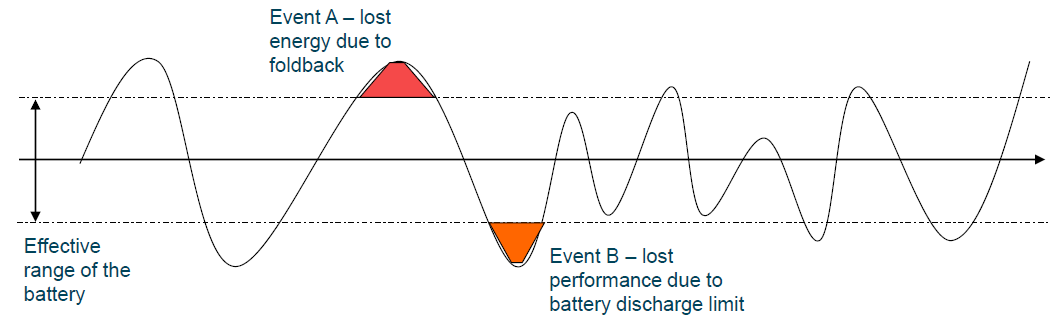
\includegraphics[width = 0.8\textwidth]{img/figure105.png}
    \caption{Battery charge and discharge cycle for hybrid vehicle.}
\end{figure}
\subsection{Energy flow diagrams of two manoeuvres}
\begin{figure}[H]
    \centering
    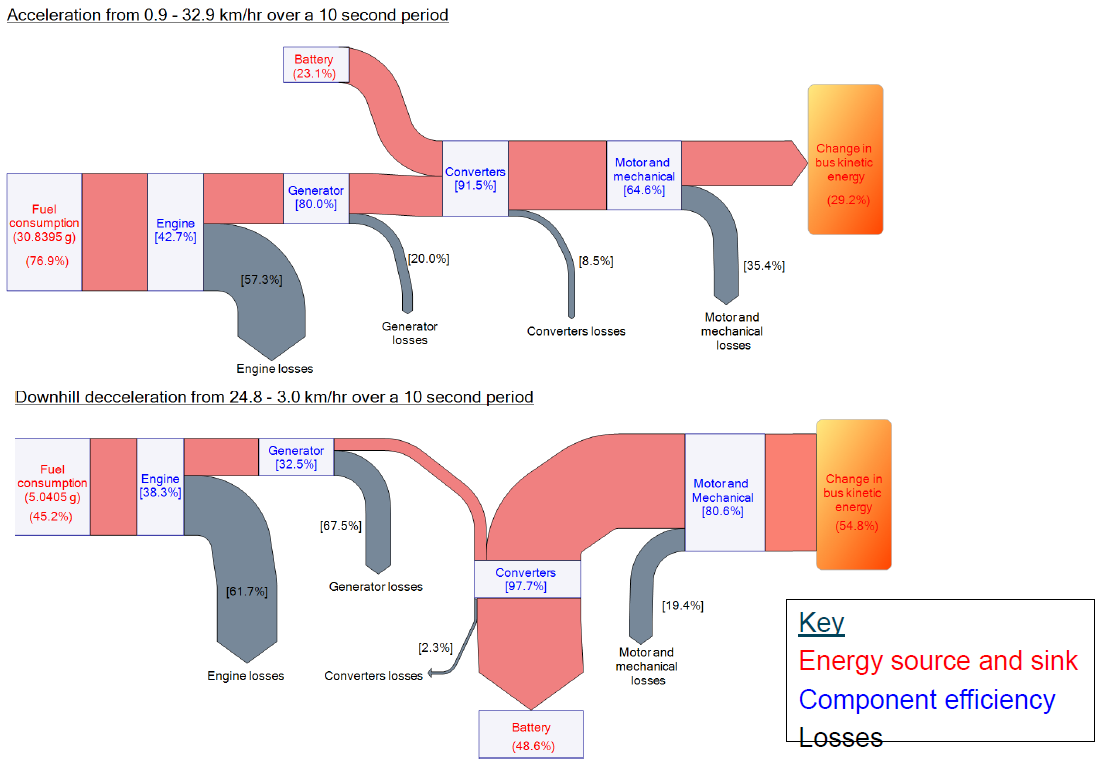
\includegraphics[width = 0.8\textwidth]{img/figure106.png}
    \caption{Energy flow diagrams of two manoeuvres.}
\end{figure}
\section{Battery electrical vehicles}
\subsection{Electric and / or hybrid vehicles?}
Domestic policy goals:
\begin{itemize}
    \item Reduce dependence on foreign oil (energy security)
    \item Job creation
    \item Economic growth (energy sources local)
\end{itemize}
Global impact:
\begin{itemize}
    \item Europe to mitigate climate change
    \item China to balance growth with pollution
    \item Governments around the world have allocated funding for clean technology
\end{itemize}
Energy independence:
\begin{itemize}
    \item Local energy sources reduce price volatility
    \item Reduce expenditure, particularly to unstable regions of the world
    \item Reduce dependence on few key regions - roughly half of the EU's gas consumption comes from only three countries (Russia, Norway, Algeria)
\end{itemize}
Developing nations:
\begin{itemize}
    \item Lower-cost conventional vehicles support economic development goals
    \item Urban air pollution and rising oil imports to be the main driver of electrification
    \item China has stated its goal of reducing the carbon intensity of its economy
    \item Lack of infrastructure (grids) is a huge factor
\end{itemize}
Climate change:
\begin{itemize}
    \item UN COPs and other aspirational organisations to reduce GHG
    \item Global support for climate change has gained momentum with Europe leading the way
    \item Transportation accounts for roughly 15\% of energy related CO2 emissions globally
    \item EU / UK energy policy provides affordable energy while contributing to the EU's wider social and climate goals
    \item Increasing legislation on reducing emissions e.g. UK to zero emissions by 2050
\end{itemize}
\subsection{Enablers - BEVs}
\begin{itemize}
    \item Increasingly stringent emissions
    \item Improving battery technologies
    \item Existing infrastructure easily expanded
\end{itemize}
\subsection{Threats}
\begin{itemize}
    \item Consumer acceptance
          \begin{itemize}
              \item Regulator pressure (lifestyle led)
              \item Acceptance of technology
          \end{itemize}
    \item Low (and relatively stable) energy prices
    \item ICE presents a difficult cost target with which to compete
\end{itemize}
\subsection{Electric: city driving losses}
\begin{figure}[H]
    \centering
    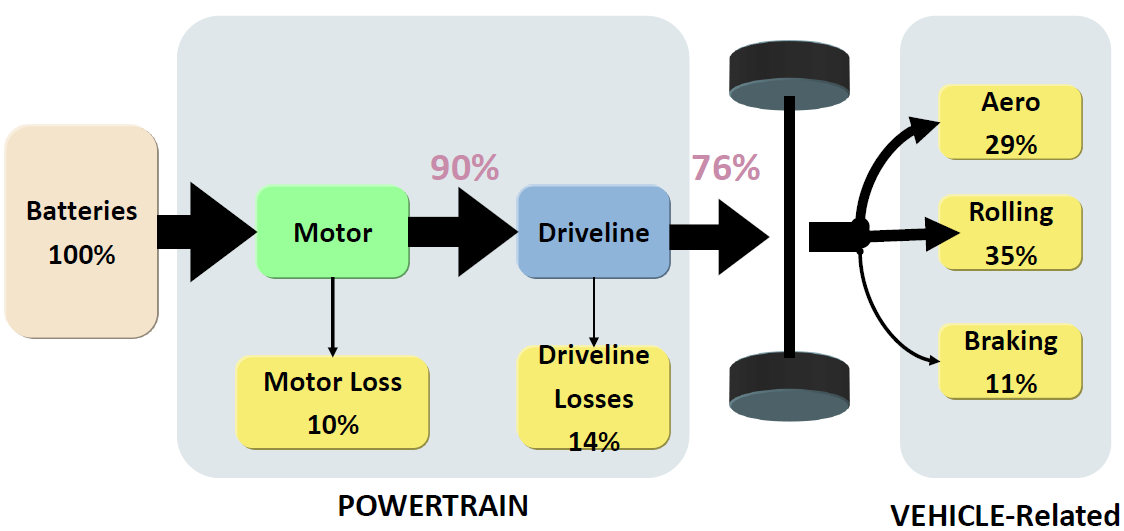
\includegraphics[width = 0.8\textwidth]{img/figure107.png}
    \caption{Electric: city driving losses.}
\end{figure}
\subsection{Energy equivalency}
\begin{figure}[H]
    \centering
    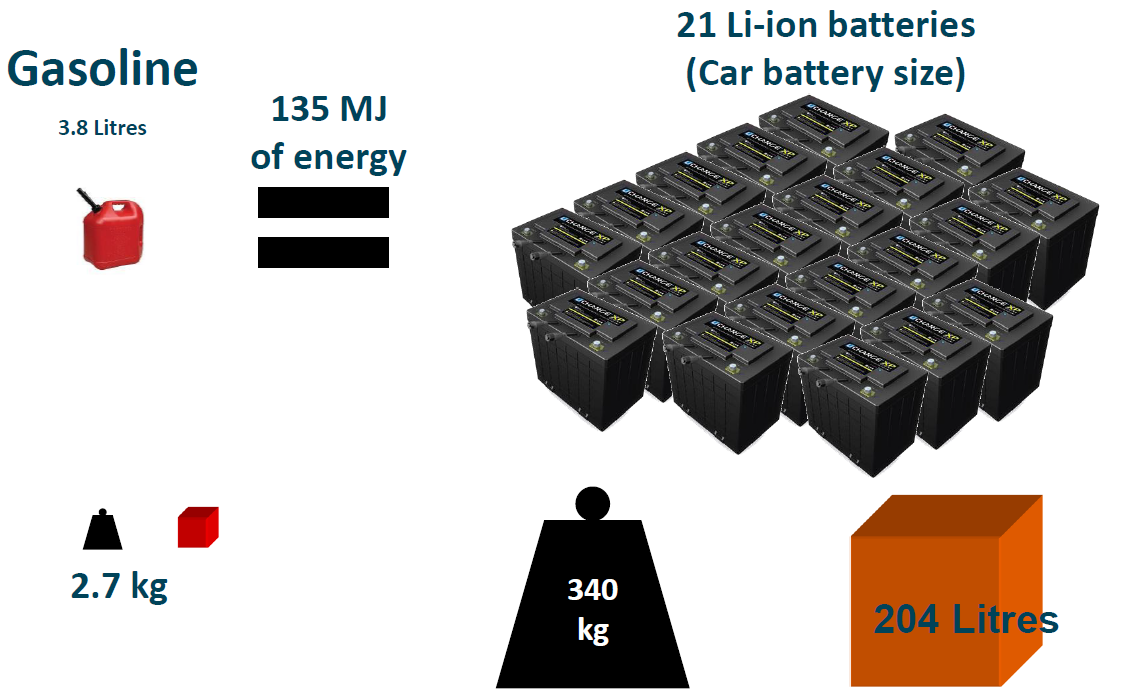
\includegraphics[width = 0.8\textwidth]{img/figure108.png}
    \caption{Energy equivalency.}
\end{figure}
\subsection{Addressing customer perception}
\begin{itemize}
    \item Accepting limited range
          \begin{itemize}
              \item Most people drive less than \SI{40}{miles\per day}
              \item Most cars are parked 23 hours of the day anyway
          \end{itemize}
    \item Smaller vehicles and reduced performance
          \begin{itemize}
              \item In the last 30 years, nearly 100\% of efficiency improvements have gone to increasing vehicle size and performance, not reducing consumption
          \end{itemize}
    \item How do y ou get people to charge at the right time
\end{itemize}
\subsection{Vehicle types}
\begin{table}[H]
    \centering
    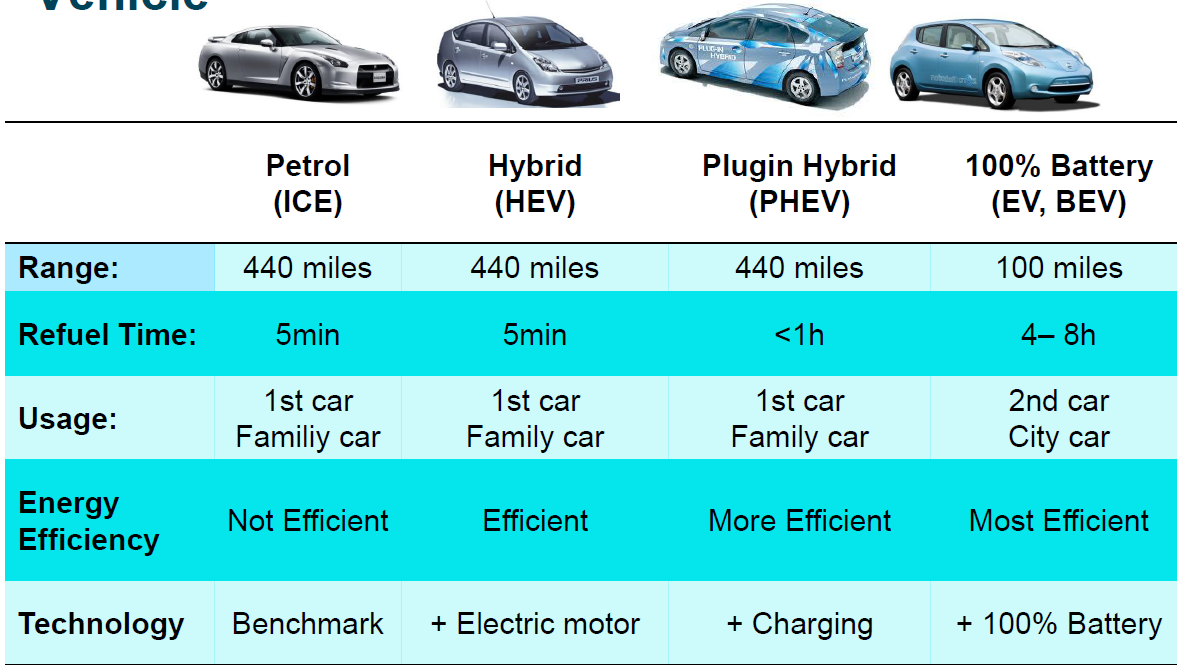
\includegraphics[width = 0.8\textwidth]{img/figure109.png}
    \caption{Vehicle types and associated performance.}
\end{table}
\subsection{Specification of typical BEV batteries}
\begin{table}[H]
    \centering
    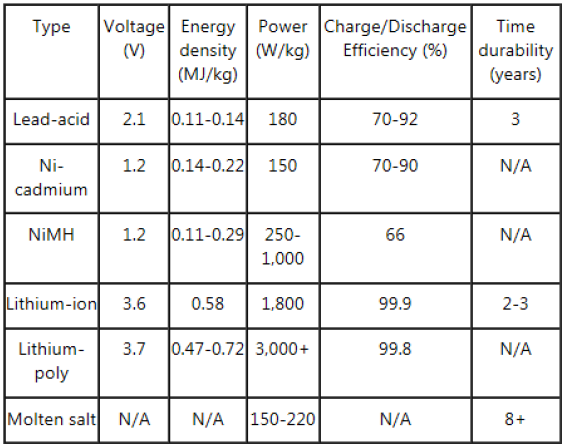
\includegraphics[width = 0.8\textwidth]{img/figure110.png}
    \caption{Specification of typical BEV batteries.}
\end{table}
Battery lifetime uncontrolled in time durability.
\subsection{Electrical vehicle - motors}
\begin{itemize}
    \item Two methods
          \begin{itemize}
              \item Motor drives the differential
              \item Motors in the wheel
          \end{itemize}
    \item Motor types
          \begin{itemize}
              \item Induction motor
              \item DC brushless motor
              \item PMSM - permanent magnet synchronous motor
          \end{itemize}
    \item Use
          \begin{itemize}
              \item To drive the vehicle over the speed range
              \item To regenerate energy when braking
          \end{itemize}
\end{itemize}
\subsection{Batteries}
\begin{itemize}
    \item Lithium sources
          \begin{itemize}
              \item We're not Lithium constrained
              \item Abundant
              \item Recyclable
          \end{itemize}
    \item Recycling - 90\% recoverable
    \item Extending battery life
    \item Battery management systems
    \item Weight / volume reductions
    \item Alternative chemistries
\end{itemize}
\subsection{Initial cost}
\begin{itemize}
    \item Companies that sell vehicles but lease the batteries
    \item Leases like power purchase agreements
          \begin{itemize}
              \item Split operating cost savings with financer
          \end{itemize}
    \item Charging infrastructure
          \begin{itemize}
              \item Charging subscription plans
          \end{itemize}
\end{itemize}
\subsection{Electrical infrastructure to support charging station infrastructure}
\begin{figure}[H]
    \centering
    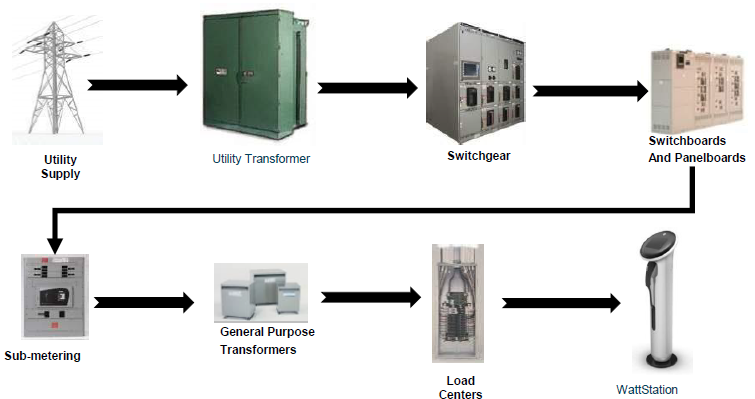
\includegraphics[width = 0.8\textwidth]{img/figure111.png}
    \caption{Energy equivalency.}
\end{figure}
\subsection{Operational / environmental metrics}
\begin{itemize}
    \item On average EV charging time has reduced from 12-18 hours to as little as 4-8 hours for a standard charge assuming a \SI{24}{kWh} battery and a full-cycle charge
    \item If 10,000 vehicle owners switched from gas-powered passenger cars to EVs, over 33,000 metric tons of CO2 emissions could be avoided annually
    \item This is equivalent to the annual CO2 emissions of approximately 6,500 gas-powered passenger cars on U.S. roads
    \item On average, an EV owner will save about 75\% of the annual fuel costs by switching from gas to electric
\end{itemize}
\section{Fuel cell vehicles}
\subsection{Hydrogen}
Hydrogen accounts for 75\% of the known universe.
\begin{quoting}
    On earth, it's not an energy source like oil or coal, only an energy carrier like electricity or gasoline, a form of energy, derived from a source and must be liberated
\end{quoting}
Much of today's hydrogen is achieved by reformed HCs or CHs with heat and catalysts or alternatively electrolysing water (split H$_2$O with electricity). In the future it may be possible to bio-tech (micro-organisms) under experimental development. \SI{1}{\kilo\gram} of H$_2$ contains same energy as 1 `U.s. gallon of gasoline' but is much lighter.
\subsection{Layout of fuel cell vehicle}
\begin{figure}[H]
    \centering
    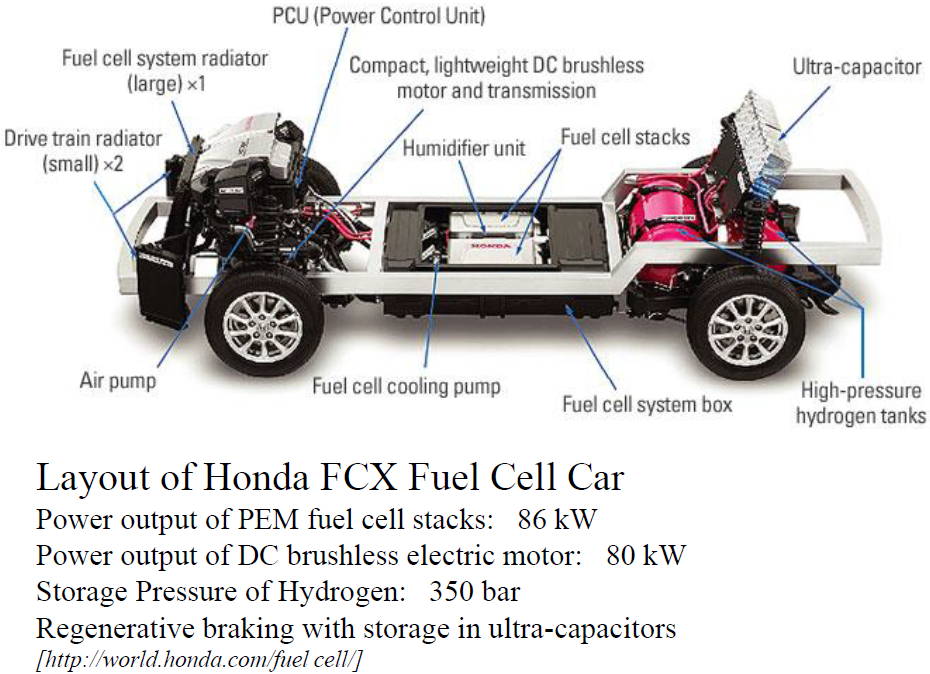
\includegraphics[width = 0.8\textwidth]{img/figure112.png}
    \caption{Layout of fuel cell vehicle.}
\end{figure}
\subsection{Fuel cell efficiency}
The efficiency of a fuel cell is limited by different considerations.
\begin{gather}
    \textrm{Max fuel cell efficiency} = \frac{\textrm{change of chemical potential for H$_2$/O$_2$ reaction}}{\textrm{change of enthalpy for H$_2$/O$_2$ reaction}}
\end{gather}
For the H$_2$/O$_2$ reaction at around atmospheric temperature, this ratio is approximately 0.83 (83\% efficiency). Unfortunately this ratio drops with temperature.
\begin{figure}[H]
    \centering
    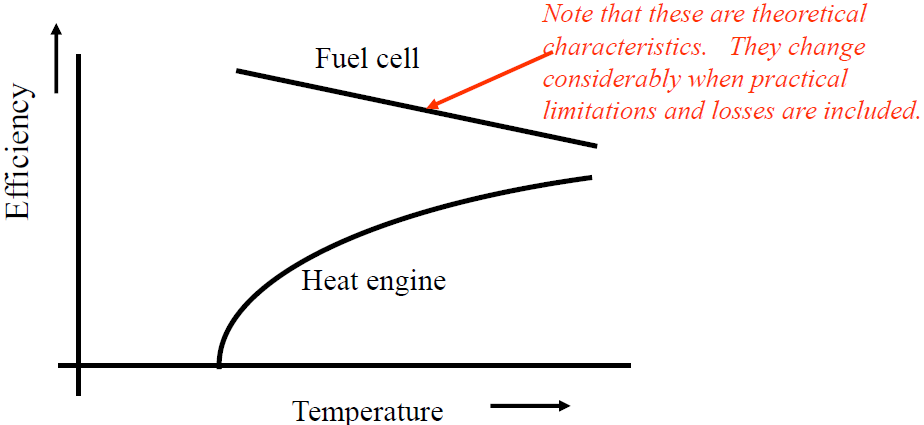
\includegraphics[width = 0.8\textwidth]{img/figure113.png}
    \caption{Fuel cell efficiency against temperature.}
\end{figure}
\subsection{Hydrogen vehicle - London RV1}
Bus performance:
\begin{itemize}
    \item 8 buses in operation
    \item \SI{35}{mph} top speed
    \item 200 miles max range
\end{itemize}
Hybrid system:
\begin{itemize}
    \item Series propulsion
    \item Supercapacitor as energy storage
    \item \SI{75}{\kilo\watt} PEM-FC
\end{itemize}
H$_2$ information:
\begin{itemize}
    \item \SI{13}{min} to refill H$_2$
    \item \SI{350}{bar}, \SI{15}{\degree C}, \SI{32}{\kilo\gram} cylinder H$_2$
    \item 200 miles max range
\end{itemize}
\begin{figure}[H]
    \centering
    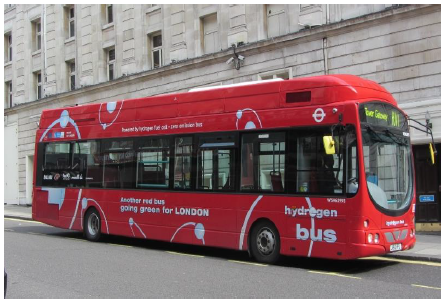
\includegraphics[width = 0.8\textwidth]{img/figure114.png}
    \caption{London RV1.}
\end{figure}
\begin{figure}[H]
    \centering
    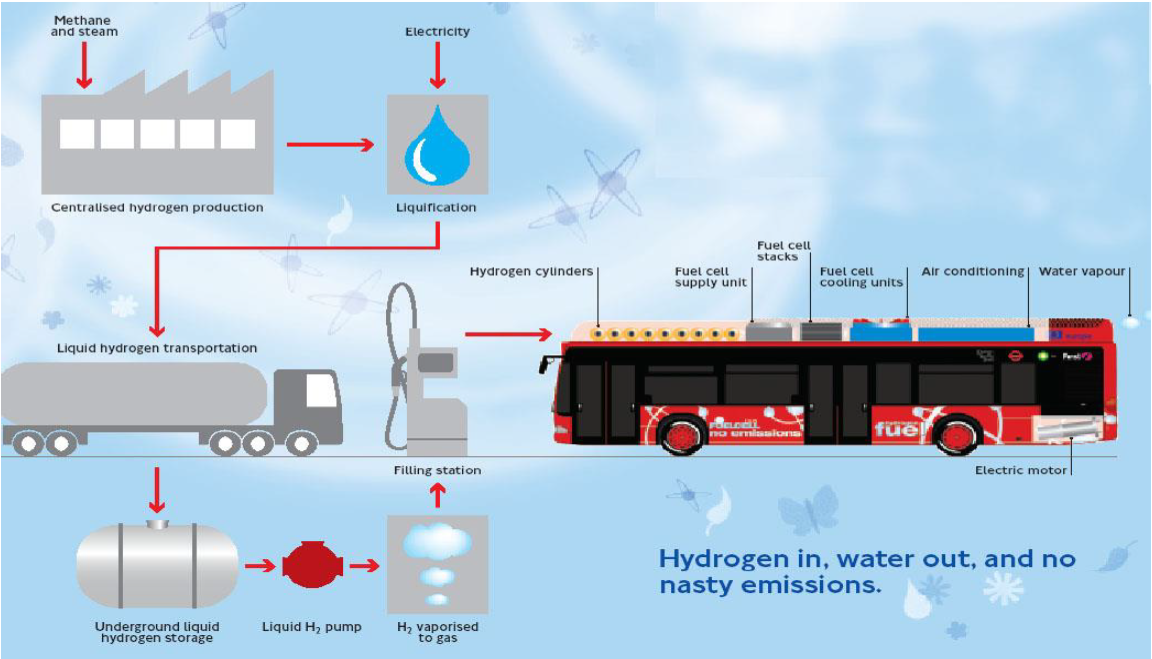
\includegraphics[width = 0.8\textwidth]{img/figure115.png}
    \caption{Supply chain for hydrogen-powered London buses.}
\end{figure}